%!TEX root = ../dokumentation.tex

\chapter{Umsetzung}

Im folgenden wird nun detailliert auf das entwickelte Konzept eingegangen und deren Funktionsweisen erläutert.

%title wird unter dem Bsp. abgedruckt
%caption wird im Verzeichnis abgedruckt
%label wird zum referenzieren benutzt, muss einzigartig sein.

\section{Voraussetzungen}
Für die Nutzung des Audioplayer auf dem Raspberry Pi bzw. für die weitere Entwicklung, müssen vorerst einige Anpassungen und Installationen getätigt werden. Diese Schritte sind notwendig damit der Audioplayer wie vorgesehen funktioniert und keine unvorhergesehen Zustände entstehen.

\subsection{Pakete installieren und Raspberry Pi updaten}
Standardmäßig besitzt der Raspberry Pi das Betriebssystem \textit{Raspbian}. Dieses gilt es zuerst auf die neuste Version zu aktualisieren. Zusätzlich werden alle installierten Pakete des System auf die neuste Version zu aktualisieren. Dieses Vorhaben wird mit den folgenden Befehlen durchgeführt:
\begin{lstlisting}[caption={Aktualsierien des Raspberry Pi}]
sudo apt-get update 
sudo apt-get upgrade 
sudo apt-get install rpi-update 
sudo rpi-update
\end{lstlisting}
Die ersten drei Befehle werden mit \ac{APT} ausgeführt. \ac{APT} ist ein Paketverwaltungssystem welches für den Bereich der Debian Betriebssysteme entwickelt wurde. Das Tool verwaltet Debian Pakete und somit auch die installierten Applikationen auf dem Raspberry Pi \autocite{apt-debian-wiki_2019}.
Zusätzlich wird für alle durchzuführende Befehle der \verb|sudo| Befehl benutzt. \ac{Sudo} wird meistens dafür benutzt bestimmte Befehle mit Root-Rechten also mit Administratorrechten auszuführen. Der Vorteil liegt darin, dass der Nutzer eben nicht ein Administrator sein muss, um kurzfristig einen Befehl als Administrator auszuführen \autocite{moeller_2013}.
Mit dem Befehl \verb|sudo apt-get update| werden alle Paketquellen neu eingelesen - also ein großes Lexikon wo man jedes Paket mit der neusten zur Verfügung stehenden Version finden kann.
Mit dem Befehl \verb|sudo apt-get upgrade| werden alle bereits installierten Paket auf die in den Paketquellen vorhandene neuste Version aktualisiert. Dabei werden keine neuen Pakete installiert oder alte nicht mehr benötigte Abhängigkeiten entfernt. \autocite{apt-get-wiki_2019}
Mit dem Befehl \verb|apt-get install rpi-update| wird das Paket \verb|rpi-update| mit allen seinen Abhängigkeiten heruntergeladen und installiert. Das Paket ist ein automatisiertes Skript zum updaten des Raspberry Pi's Betriebssystem auf die neuste Version.
Als letzten Schritt wird nun das Paket \verb|rpi-update| ausgeführt und der Raspberry Pi lädt automatisch das neuste passende Betriebssystem herunter und installiert es. Dabei gehen keine Daten verloren.
\\
Nachdem der Raspberry Pi sich erfolgreich aktualisiert hat, müssen nun noch die jedenfalls benötigten Pakete installiert werden. Dies wird mit den folgenden Befehlen gemacht.
\begin{lstlisting}[caption={Installation benötigter Pakete}]
sudo apt-get install portaudio19-dev
sudo apt-get install libmpg123-dev
sudo apt-get install mp3info 
\end{lstlisting}

\subsection{Nötige Schritte für Entwicklungszwecke}
Im folgenden wird auf die einzelnen Schritte eingegangen, die nötig sind um an dem erstellten Programm weiter zu entwickeln. Dazu müssen die im Anschluss stehenden Befehle auf dem Raspberry Pi ausgeführt werden.
\subsubsection{Installieren von Go}
Nun wird auf die Installation von Go eingegangen.
\begin{enumerate}
\item \textbf{Herunterladen von Go}  \\
Als ersten Schritt gilt es die Programmiersprache Go auf den Raspberry Pi herunterzuladen. Dazu stellt der Hersteller offizielle Pakete für die unterschiedlichen Betriebssysteme und Architekturen zum Download bereit. Diese können über die \href{https://golang.org/dl/}{Download-Webseite} heruntergeladen werden. In diesem Fall wird für den Raspberry Pi das Paket für das Betriebssystem \textit{Linux} mit der Architektur \textit{ARMv6} benötigt. Nachdem das passende Paket auf der Webseite gefunden wurde, muss der Direkt-Link zu dem Download in den Zwischenspeicher kopiert werden und anschließend der folgende Befehl auf dem Raspberry Pi ausgeführt werden.
\begin{lstlisting}
Befehl: wget [LINK]
\end{lstlisting}

\item \textbf{Entpacken des Archivs}  \\
Nachdem das offizielle Archiv für die Programmiersprache Go heruntergeladen wurde, muss dieses nun nach den Pfad \verb|/user/local| entpackt werden. Für das entpacken des Archivs wird das standardmäßige Archivierungsprogramm für Linux \textit{\ac{Tar}} verwendet. Der große Vorteil eines tar-Archivs ist, dass die Benutzerrechte einer Datei mit gesichert werden und diese beim Entpacken auch wiederhergestellt werden \autocite{tar-wiki_2019}. Das entpacken des Archivs wird durch den folgenden Befehl realisiert. Der Dateiname entspricht hier der zuvor heruntergeladenen Datei.
\begin{lstlisting}
tar -C /usr/local -xzf [Filename]
\end{lstlisting}

\item \textbf{Setzen des Export-Pfad} \\
Damit das Betriebssystem Go auch System weit kennt, muss der Pfad zu der ausführbaren Datei von Go in die PATH-Variable eingetragen werden. Die \textit{PATH-Variable} ist eine Umgebungsvariable, die aus einer Komma-separierten Liste von Ordnern besteht, die die Shell beim der Eingabe eines Kommandos durchsucht \autocite{quigley_2000}. Dies bewirkt, dass von jedem Standpunkt im System auf Go bzw. den Go Compiler zugegriffen werden kann.
\begin{lstlisting}
export PATH=\$PATH:/usr/local/go/bin
\end{lstlisting}

\item \textbf{Überprüfen der Go Installation auf Korrektheit} \\
Um nun zu Überprüfen, ob Go richtig installiert wurde und die Path-Variable korrekt gesetzt wurde, wird nun durch den einfachen Befehl \verb|go version| eine Abfrage an den Go Compiler zu seiner aktuellen Version erstellt. Wird dabei eine gewisse Version angezeigt, ist Go richtig installiert und im System integriert.
\begin{lstlisting}
go version -> "go version go x.x.x"
\end{lstlisting}

\item \textbf{Go-Ordnerstruktur anlegen} \\
Go empfiehlt es eine Gewisse Ordnerstruktur für die Go Projekte anzulegen. Diese mit den folgenden Befehlen angelegt und besteht aus:
\begin{itemize}
\item \textbf{bin} - enthält alle Go-Executable's, die mit dem Befehl \verb|go install| installiert wurden.
\item \textbf{pkg} - enthält alle kompilierten Pakete, die in Projekte importiert werden können. 
\item \textbf{src} - enthält alle Quelldateien, entweder die eigenen oder aus externen Repositories heruntergeladene Quellen.
\end{itemize}
In der folgenden Übersicht wird die Ordnerstruktur nochmals visuell dargestellt.
Der Ordner \textit{pi} stellt hier den Nutzernamen da, der sich bei jedem System natürlich unterscheiden kann. \\
\begin{minipage}[t]{\textwidth}
\dirtree{%
.1 /. 
.2 home. 
.3 pi. 
.4 go. 
.5 src. 
.5 pkg. 
.5 bin. 
}
Die Befehle zur Erstellung der Ordnerstruktur sehen wie folgt aus. \\
Ausgehend von \verb|$Home|:
\begin{lstlisting}[caption={Erstellung der Go Ordnerstruktur}]
mkdir go
cd go
mkdir src
mkdir pkg
mkdir bin
\end{lstlisting}
\end{minipage}


\end{enumerate}

\subsubsection{Klonen des Git Repository}
Der nächste Schritt ist das Git Repository auf den lokalen PC zu klonen. Go schreibt dafür einen Standard vor, wie die Ordnerstruktur dazu bestenfalls aufgebaut werden sollte. Im folgenden werden nun die Befehle zur Erstellung Ordnerstruktur dargestellt. 
Diese Befehle Starten von \verb|/home/pi/go/src/| :
\begin{lstlisting}[caption={Klonen des Git Repository}]
mkdir github.com 
cd github.com
mkdir alexanderklapdor
cd alexanderklapdor
git clone https://github.com/alexanderklapdor/RaspberryPi_Go_Audioplayer.git
\end{lstlisting}

\subsubsection{Installieren der Go Abhängigkeiten}
Bei der Entwicklung des Audioplayers wurden weitere Go-Projekte verwendet, welche nun für die Entwicklung auf den lokalen Rechner heruntergeladen werden müssen. Um nicht alle Abhängigkeiten einzeln zu installieren, kann Go sich alle benötigten Projekte alleine herunterladen. Dies wird durch den folgenden Befehl gemacht.
Starting from \verb|../RaspberryPi_Go_Audioplayer/| :
\begin{lstlisting}
go get ./...  
\end{lstlisting}

\subsubsection{Modifizieren der ALSA Bibliothek Dateien}
Die Konfigurationdatei der ALSA Bibliothek muss editiert werden damit die Fehlermeldungen, welche durch die nicht vorhandenen Anschlüsse am Raspberry Pi hervorgerufen werden, nicht immer mit ausgegeben werden. \\
Zugriff auf die Datei wird mit dem Befehl \verb|sudo nano /usr/share/alsa/alsa.conf|  \\
Folgende Einträge müssen aus dieser Datei entfernt werden:
\begin{lstlisting}[caption={Liste der zu löschenden Einträge}]
pcm.rear cards.pcm.rear 
pcm.center_lfe cards.pcm.center_lfe 
pcm.side cards.pcm.side 
pcm.surround21 cards.pcm.surround21 
pcm.surround40 cards.pcm.surround40 
pcm.surround41 cards.pcm.surround41 
pcm.surround50 cards.pcm.surround50 
pcm.surround51 cards.pcm.surround51 
pcm.surround71 cards.pcm.surround71 
pcm.iec958 cards.pcm.iec958 
pcm.spdif iec958 
pcm.hdmi cards.pcm.hdmi 
pcm.dmix cards.pcm.dmix 
pcm.dsnoop cards.pcm.dsnoop 
pcm.modem cards.pcm.modem 
pcm.phoneline cards.pcm.phoneline
\end{lstlisting}

\subsection{Nötige Schritte für die Nutzung}
Für die reine Nutzung des Audioplayer sind durchaus weniger Schritte notwendig, da eine bereits kompilierte Version heruntergeladen und genutzt werden kann.
Dazu sind folgende Schritte notwendig:
\begin{enumerate}
\item \textbf{Herunterladen der neusten \href{https://github.com/alexanderklapdor/RaspberryPi_Go_Audioplayer/releases}{Release} Datei}  \\
\begin{lstlisting}
wget [LINK]
\end{lstlisting}

\item \textbf{Entpacken des Archiv} \\
\begin{lstlisting}
tar -xvf RaspberryPi_Go_Audioplayer_v***.tar
\end{lstlisting}

\item \textbf{Starten des Audioplayers} \\
\begin{lstlisting}
./RaspberryPi_Go_Audioplayer_v***/MusicPlayerClient
\end{lstlisting}
\end{enumerate}

\section{Konzept}
Hier wird das allgemeine/übergeordnete Konzept dargestellt. Das muss dann hier auch noch genau erläutert werden wie das funktioniert, mit dem Hinweis, dass auf die einzelnen Punkte wie Client, Server und Socket im nach hinein nochmals explizit eingegangen wird
\begin{figure}[h]
	\centering
	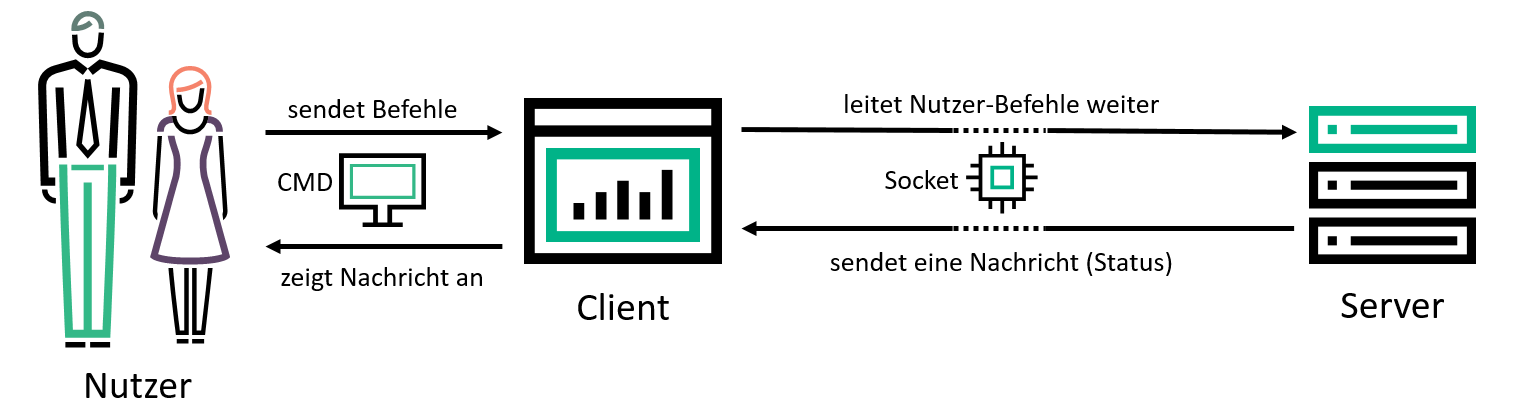
\includegraphics[scale=0.5]{Audioplayer_Konzept.png}
	\caption{Audioplayer - Konzept}
	\label{img:grafik-RaspberryPi3}
\end{figure}
\newline

\subsection{Konzept des Clients}
Im folgenden wird nun auf den Client explizit eingegangen...hier sieht man den Ablauf der Hauptfunktion Funktion des Clients.

\begin{figure}[H]
    \begin{struktogramm}(160,75)[Main-Funktion] 
        \assign{\hfill Konfigurationsdatei auslesen\hfill} 
        \assign{\hfill Aufsetzen des Loggers\hfill}
        \ifthenelse[12]{2}{1} {Überprüfen ob Server bereits läuft}{Ja}{Nein} 
        	\change
            \assign[5]{\hfill Starten des Servers\hfill}
        \ifend
        \ifthenelse[15]{2}{1} {Überprüfen ob Übergabeparameter übergeben wurden}{Ja}{Nein} 
        	\assign{\hfill Parsen der Informationen in ein JSON Format\hfill}
            \assign{\hfill Senden des JSONs and den Server\hfill}
            \while[5]{Bis Nachricht vom Server kommt}
            	\assign{\hfill Warten...\hfill}
            \whileend
            \assign{\hfill Anzeigen der Nachricht vom Server\hfill}
            \change
        \ifend
        \assign[5]{\hfill Beenden des Clients\hfill}
    \end{struktogramm} 
\caption{Client Programm - Ablauf} 
\label{lst:client_ablauf} 
\end{figure}

\subsection{Konzept des Servers}

Im folgenden wird nun auf den Server explizit eingegangen...hier sieht man den Ablauf der Hauptfunktion Funktion des Server.

\begin{figure}[H]
    \begin{struktogramm}(160,80)[Main-Funktion] 
        \assign{\hfill Konfigurationsdatei auslesen\hfill} 
        \assign{\hfill Aufsetzen des Loggers\hfill}
        \assign{\hfill Aufsetzen des Sockets\hfill}
        \assign{\hfill Starten des Pulseaudio Servers\hfill}
        \while[5]{Endlosschleife}
        	\assign{\hfill Abhören des Sockets auf Nachrichten\hfill}
        	\ifthenelse[12]{5}{1} {Nachricht erhalten}{Ja}{Nein}
        	    \assign[5]{\hfill Entpacken der Nachricht\hfill}
        	    \ifthenelse[12]{6}{5} {Befehl == \enquote{Beenden}}{Ja}{Nein}
        	    	\assign[5]{\hfill Nachricht an Client senden\hfill}
        	    	\assign[5]{\hfill Beenden des Pulseaudio Server\hfill}
        	    	\assign[5]{\hfill Schließen des Sockets\hfill}
        	    	\assign[5]{\hfill Beenden des Servers\hfill}
        	    	\change
        	    	\assign[10]{\hfill Ausführen des Befehls\hfill}
        	    	\assign[10]{\hfill Nachricht an Client senden\hfill}
        	    \ifend
        		\change
        	\ifend
        \whileend
    \end{struktogramm} 
\caption{Server Programm - Ablauf} 
\label{lst:server_ablauf} 
\end{figure}
	

\section{Kommunikation über Sockets}
Eines der größten Schwierigkeiten in diesem Projekt war es ein Programm zu entwickeln, was einerseits eine Audiodatei abspielt und gleichzeitig noch Befehle entgegennehmen kann jedoch dazu aber nicht das System blockiert, sodass nichts anderes mehr getätigt werden kann. Um dies zu ermöglichen wurde sich für das bereits beschriebene Konzept aus Server und Client entschieden, die über einen Socket kommunizieren. \\
Ein \textit{Socket} ist ein Kommunikationsendpunkt der vom Betriebssystem als Objekt bereitgestellt wird. Programme verwenden meistens Sockets um mit anderen Programmen Daten auszutauschen und miteinander zu kommunizieren. Dies ist unabhängig davon, ob beide Programme sich auf dem selbem Computer oder einem anderen, über das Netzwerk erreichbaren Computer befinden. Sockets kommunizieren in der Regel bidirektional, was bedeutet, dass über den Socket sowohl Daten gesendet wie auch empfangen werden können. Technisch ist der Socket ein Speicherbereich in dem Konfigurationsparameter einer Verbindung wie auch ankommende und abgehende Daten zwischengespeichert werden. Aufgrund dessen, dass ein Socket vom Betriebssystem bereit gestellt wird, hat man keinen direkt zugriff auf den Socket sondern kann nur über Funktionen der Programmiersprache auf den Socket zugreifen.
Ein Socket wird immer von einem Programm bei Bedarf erstellt und ist somit diesem Prozess fest zugeordnet \autocite{pollakowski_2012}. \\
Dies erlaubt es, dass der Server im Hintergrund Befehle entgegennehmen und Audio Dateien abspielen kann und dabei nicht das System "blockiert". Der Client der über den Socket mit dem Server kommuniziert wird immer nur für die Übertragung eines Befehl übertragen und hat damit nur die Aufgabe den Server mit neuen Befehlen zu füllen.

\section{Funktionen des Programms}
Hier kommen die Scheiß Funktionen rein, alle Beschreiben und vll. kurz erläutern evtl. an einer Zeichnung wie diese Ablaufen.

\href{https://github.com/alexanderklapdor/RaspberryPi_Go_Audioplayer#commands-of-the-client}{Kommandos}
\\
\href{https://github.com/alexanderklapdor/RaspberryPi_Go_Audioplayer#console-arguments}{Console-Arguments}


\section{Bedienung des Programms}
Beispiele für die Bedienung reinmachen ( Ordner abspielen, Loop, Playlist, blabla)

